% User guide: http://mirrors.ctan.org/macros/latex/contrib/bookcover/bookcover.pdf
% A4 size 210 x 297 mm
\documentclass[
    coverwidth=213mm, %150mm,
    coverheight=303mm, %200mm,
    spinewidth=17.8mm, % 289 pages, 米色道林紙 100g
%    flapwidth=6cm,
%    wrapwidth=5mm,
%    trimmed % Show only trimmed part!
    bleedwidth=3mm,
    12pt,
    trimmed=false
    ]{bookcover}

%\bookcovertrimmedpart{front} % Trimmed part is the front cover
%\bookcovertrimmedpart{back} % Trimmed part is the back cover
%\bookcovertrimmedpart{spine} % Trimmed part is the spine

\newbookcovercomponenttype{center rotate}{
    \vfill
    \centering
    \rotatebox[origin=c]{-90}{#1}
    \vfill}

\usepackage[outline]{contour}% It doesn't work with xelatex and lualatex
\contourlength{1pt}
\usepackage[english]{babel}
\usepackage{kantlipsum,microtype}

\begin{document}

\begin{bookcover}

% Remark
%\begin{bookcoverelement}{center}{above front}
%    \textcolor{blue}{A dust jacket example}
%\end{bookcoverelement}

% Background color on the whole cover
\begin{bookcoverelement}{color}{bg whole}
    white
\end{bookcoverelement}

% Background picture on the whole cover without flaps
\begin{bookcoverelement}{picture}{bg whole without flaps}
    %./figures/bookcover-bg.jpg
\end{bookcoverelement}

% Transparent areas on the back cover
%\begin{bookcoverelement}{tikz}{bg back and wrap}
%    \fill[opacity=0.3,black!50] 
%    (0,0) rectangle (25mm,\partheight) 
%    (part.north east) rectangle ([xshift=-5cm]part.south east);
%\end{bookcoverelement}

% Transparent areas on the front cover
%\begin{bookcoverelement}{tikz}{bg front and wrap}
%    \fill[opacity=0.3,black!50] 
%    (0,0) rectangle (50mm,\partheight) 
%    (part.north east) rectangle ([xshift=-25mm]part.south east);
%\end{bookcoverelement}

% Picture on the front cover behind the title
\begin{bookcoverelement}{center}{front}
    
\includegraphics{watermarkTMU.jpg}
    %{./figures/bookcover-cards.pdf}
\end{bookcoverelement}

% Author and title on the front cover
\begin{bookcoverelement}{normal}{front}[,,,5cm]
    \centering % yellow!60!
    \color{black}\sffamily\bfseries
    \resizebox{!}{5mm}{
    %\contour{black}{}
    Taipei Medical University}\\[20mm]
    \resizebox{!}{7mm}{%\contour{black}{}
    Translational Medicine
    }\\[6mm]
    \resizebox{!}{7mm}{
    Dissertation of Doctor of Philosophy
    %The Ph.D. Program for 
    }\\[110mm]
    \parbox{160mm}{ %linewidth=
    {\bfseries\large 
    Global Transcriptomics and Proteomics Analyses for Biomarker Identification and Validation in Head and Neck Squamous Cell Carcinoma}}\\[40mm]
    \resizebox{!}{5mm}{
    Author: Li-Hsing Chi}\\[5mm]
    \resizebox{!}{5mm}{
    Advisors: 
    Yu-Chuan (Jack) Li,
    Michael Hsiao}\\[7mm]
    \resizebox{!}{5mm}{
    \small 2022.01}\\[26mm]

%\author{Li-Hsing Chi}
%\degreemonth{January}
%\degreeyear{2022} 
%\dissertation
%\doctorphilosophy
%%% \normalsize
%\noindent {\bf{Primary Advisors:}} 
%Yu-Chuan (Jack) Li,
%\indent\indent\indent\indent\indent\indent
%Michael Hsiao\\
%{\bf{Secondary Advisor:}} 
%Alexander TH Wu\\
\end{bookcoverelement}



% Title on the spine
\begin{bookcoverelement}{center rotate}{spine}
    %\color{yellow!60!black}
    \huge\sffamily\bfseries
    %\contour{black}
    {Li-Hsing Chi -- Bioinformatic Study of HNSCC -- 2022.01}
\end{bookcoverelement}

%%
% Text on the back cover
\begin{bookcoverelement}{normal}{back}[2cm,2cm,2cm,2cm]
    \color{gray}%\kant[1]
    %\begin{keywords}
{\large KEYWORDS:\\}
Head and Neck Squamous Cell Carcinoma (HNSCC),
Biomedical Informatics,
Forensic Medicine,
TCGA,
RNA-sequencing,
Survival Analysis,
Optimal Cutoff, Sliding-window Cutoff,
Kaplan--Meier Survival Analysis, Cox Proportional Hazard Model,
Biomarker,
%Tumor Type-agnostic Therapy,
%Immuno-Oncology,
%Targeted Therapy,
Systemic Therapy,
Surgical Margin,
Tobacco, Betel nut,
Rstudio, R, C++, Deep Learning,
Holistic Cancer Care,
%Therapeutic Relationship,
Mindfulness Meditation,
Thymosin Beta-4 X-linked (TMSB4X), %\capitalisewords{}
Calcium/calmodulin Dependent Protein Kinase II Inhibitor 1 (CAMK2N1),
Calmodulin like 5 (CALML5),
Fc Fragment of IgG Binding Protein (FCGBP)

\end{bookcoverelement}

% Text and picture on the front flap
%\begin{bookcoverelement}{normal}{front flap}[1cm,1cm,1cm,2cm]
%    \color{white}\kant[2]
%    \vfill
%    {\centering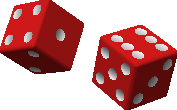
\includegraphics{./figures/bookcover-dice.pdf}\par}
%\end{bookcoverelement}

% Text on the back flap
%\begin{bookcoverelement}{normal}{back flap}[1cm,2cm,1cm,2cm]
%    \color{white}\kant[3]
%\end{bookcoverelement}

\end{bookcover}

\end{document}